\documentclass{article}
\usepackage{graphicx,float}
\usepackage{amsmath,latexsym,amsfonts,amssymb,amsthm}
\usepackage{hyperref}

\usepackage[utf8]{inputenc}
\usepackage[english]{babel}
\usepackage[letterpaper,top=2cm,bottom=2cm,left=3cm,right=3cm,marginparwidth=1.75cm]{geometry}
\renewcommand{\baselinestretch}{1.667}


\title{Compute Intelligence Lab 4 PS s7}
\author{Joris Plaščinskas}
\date{\today}


\begin{document}


\maketitle
\section*{Data}
I chose to use flower classification dataset. Dataset was split 80/10/10 into train, validation and test sets. \href{https://www.kaggle.com/datasets/sauravagarwal/flower-classification}{DATA SET LINK}. The dataset contains 5 species of flowers and in total 3540 labeled images (daisy - 607, dandelion - 872, roses - 615, sunflowers - 673, tulips - 773).

\section*{Neural Net Architecture and Data Split}
\begin{figure}[H]
    \centering
    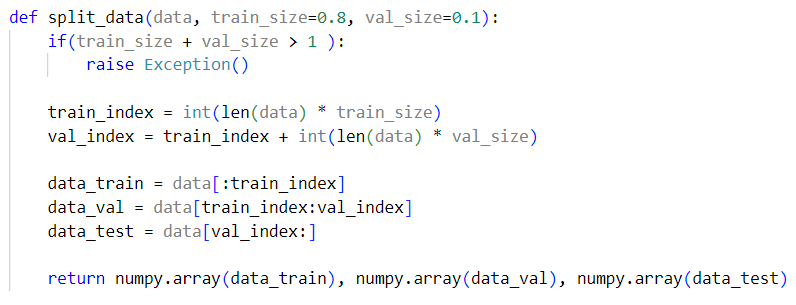
\includegraphics[width=1\textwidth]{data-split.png}
    \caption{Data Split Function}
    \label{fig:data-split}
\end{figure}
Data is first indexed, then shuffled, then read from disk and finally split into train, validation and test. Figure~\ref{fig:data-split} shows the function that is used to split data set, the first 80\% becomes train, next 10\% is split and last 10\% is test. It's important to shuffle the entries before splitting the data this way.
\begin{figure}[H]
    \centering
    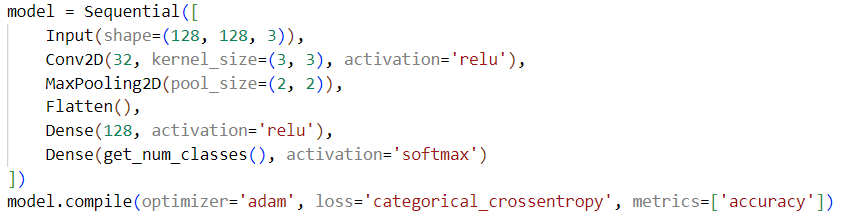
\includegraphics[width=1\textwidth]{architecture-0.png}
    \caption{Model Architecture v0}
    \label{fig:architecture-0}
\end{figure}
The simplest model (version 0) can be seen in Figure~\ref{fig:architecture-0}. It has an input of size (128, 128, 3) - the size of a processed image, a convolutional layer that detects certain features in a (2,2) size window throughout the whole image, a max pooling layer that simplifies the data by taking the maximum values in a (2, 2) window. The Flatten layer turns the 3D image data structure into a 1D vector and dense layer is just a classic feed forward neural network layer. I used the most popular - adam optimizer for training and categorical cross-entropy function for training. 
\begin{figure}[H]
    \centering
    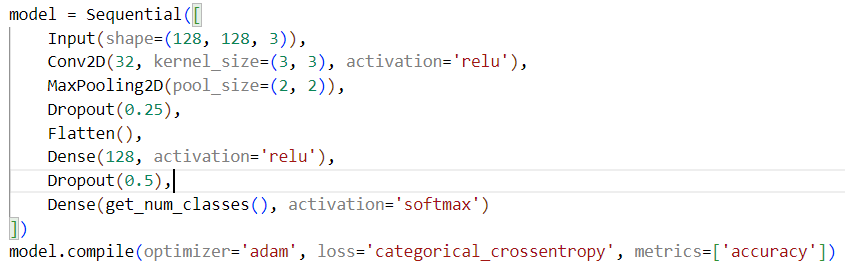
\includegraphics[width=1\textwidth]{architecture-1.png}
    \caption{Model Architecture v1}
    \label{fig:architecture-1}
\end{figure}
The version 1 model can be seen in Figure~\ref{fig:architecture-1}. It's almost the same as the 0th version, but this model also features two dropout layers to combat over-fitting. The dropout fights over-fitting by removing random neurons during training.
\begin{figure}[H]
    \centering
    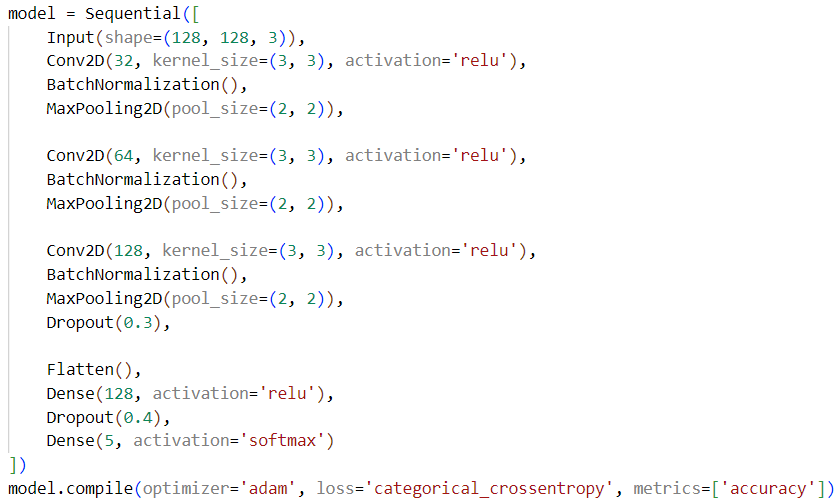
\includegraphics[width=1\textwidth]{architecture-2.png}
    \caption{Model Architecture v2}
    \label{fig:architecture-2}
\end{figure}
The final version (2) can be seen in Figure~\ref{fig:architecture-2}. I increased the model size and layer count and introduced a batch normalization layer which helps speed up the learning process by normalizing the activations of each layer.
\begin{figure}[H]
    \centering
    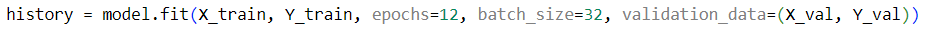
\includegraphics[width=1\textwidth]{training.png}
    \caption{Training Method}
    \label{fig:training}
\end{figure}
To train the model I simply used the built in tensorflow 'fit' method (Figure~\ref{fig:training}). Which under the hood relies on iterative optimization of the categorical cross-entropy loss function using the adam optimizer.

\section*{Data Pre-processing}
I downloaded the flowers dataset into my hard-drive, then using windows ui I removed the validation and test folders, because I decided that I will use train set for everything. I put each class folder into data folder. During the execution of my python code I first scan the directories and create two lists: X - for storing image paths, Y - for storing image labels. The two lists are then shuffled in the same order and finally image paths are replaced with actual images, which are preprocessed to be 128 x 128. The string labels are also one-hot encoded. All data pre-processing functions can be seen in Figure~\ref{fig:preprocess}.
\begin{figure}[H]
    \centering
    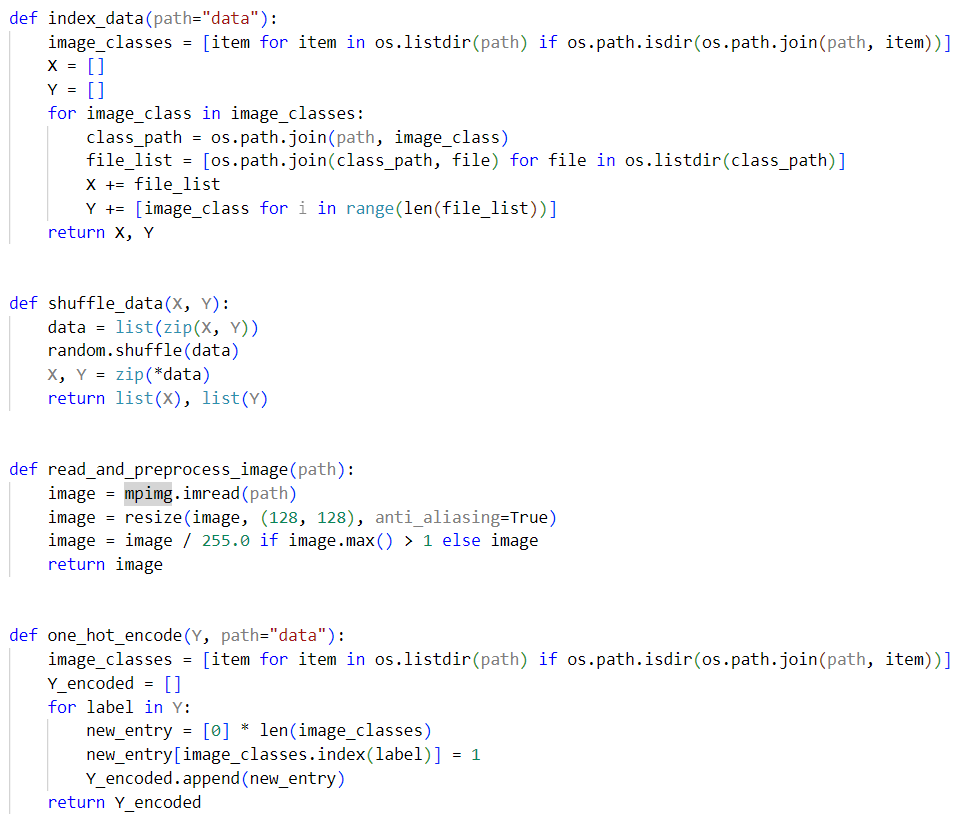
\includegraphics[width=1\textwidth]{preprocess.png}
    \caption{Data Pre-Processing}
    \label{fig:preprocess}
\end{figure}

\section*{Computational Resources}
I used CPU for processing data and a lot of RAM because all images were loaded to memory at once.

\section*{Results}
\begin{figure}[H]
    \centering
    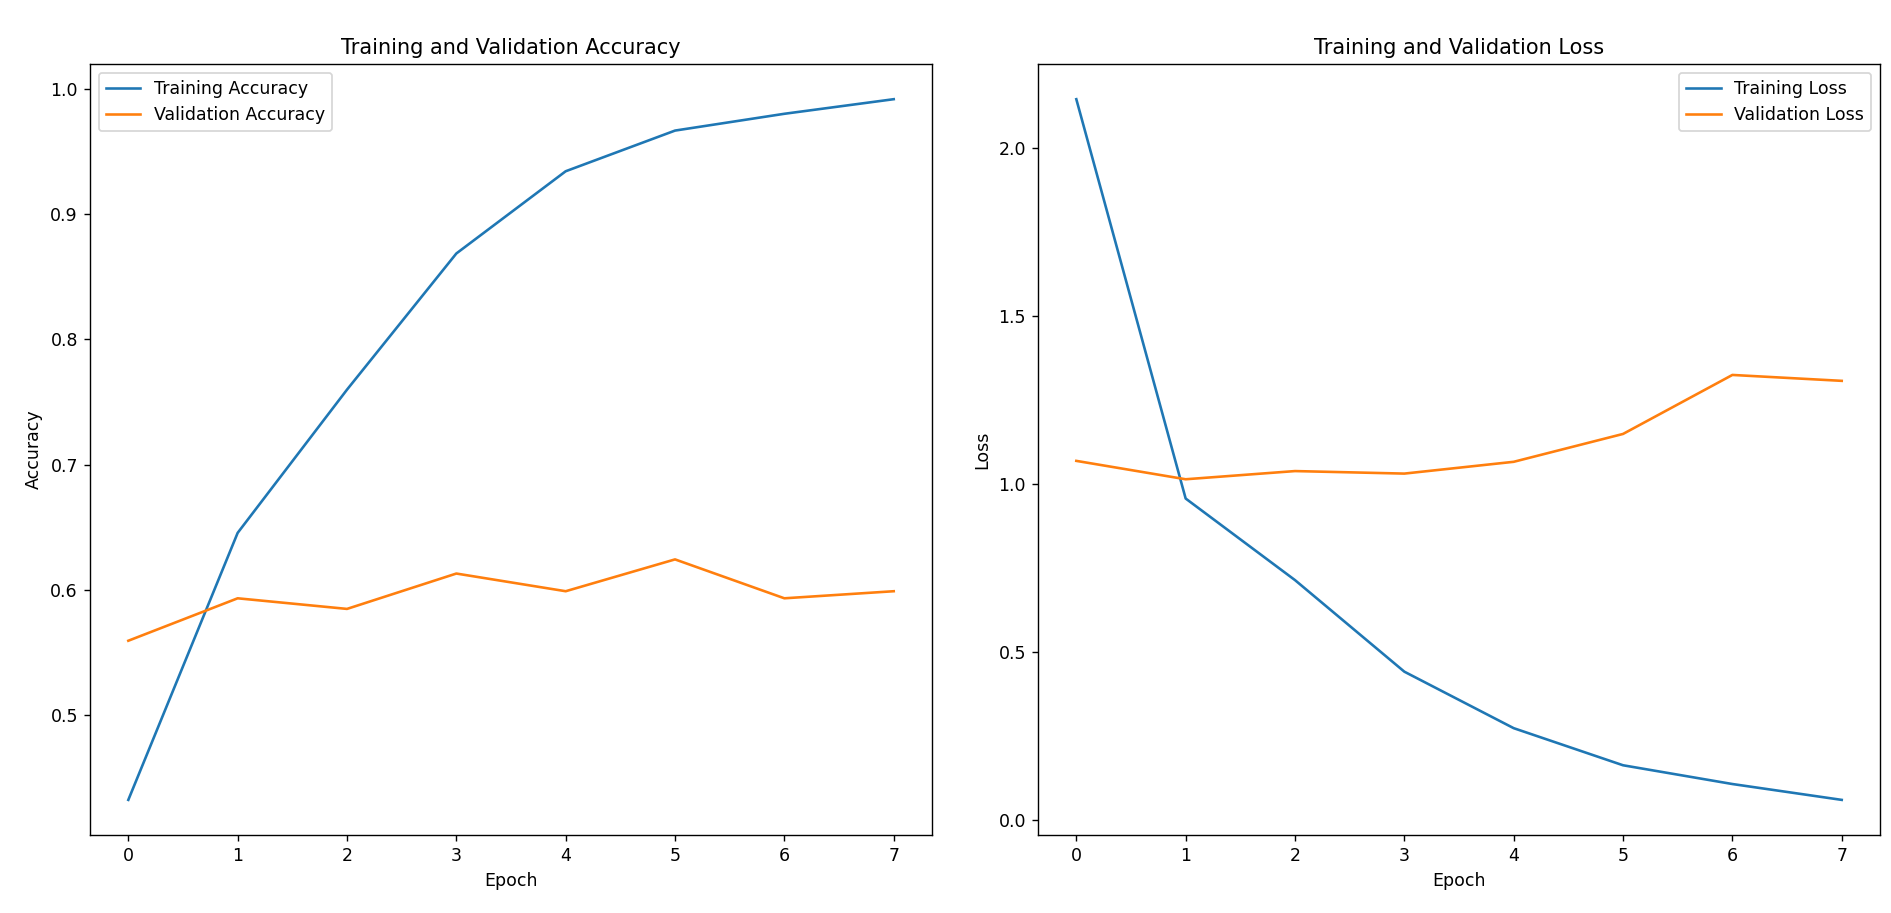
\includegraphics[width=1\textwidth]{results-0.png}
    \caption{Architecture v0 Results}
    \label{fig:results-0}
\end{figure}
In Figure~\ref{fig:results-0} are the results of training/validation sets accuracy and loss after 8 epochs of training on architecture v0. The results clearly show that the model tends to over-fit, because the training loss is significantly lower than validation loss and validation loss is even increasing.
\begin{figure}[H]
    \centering
    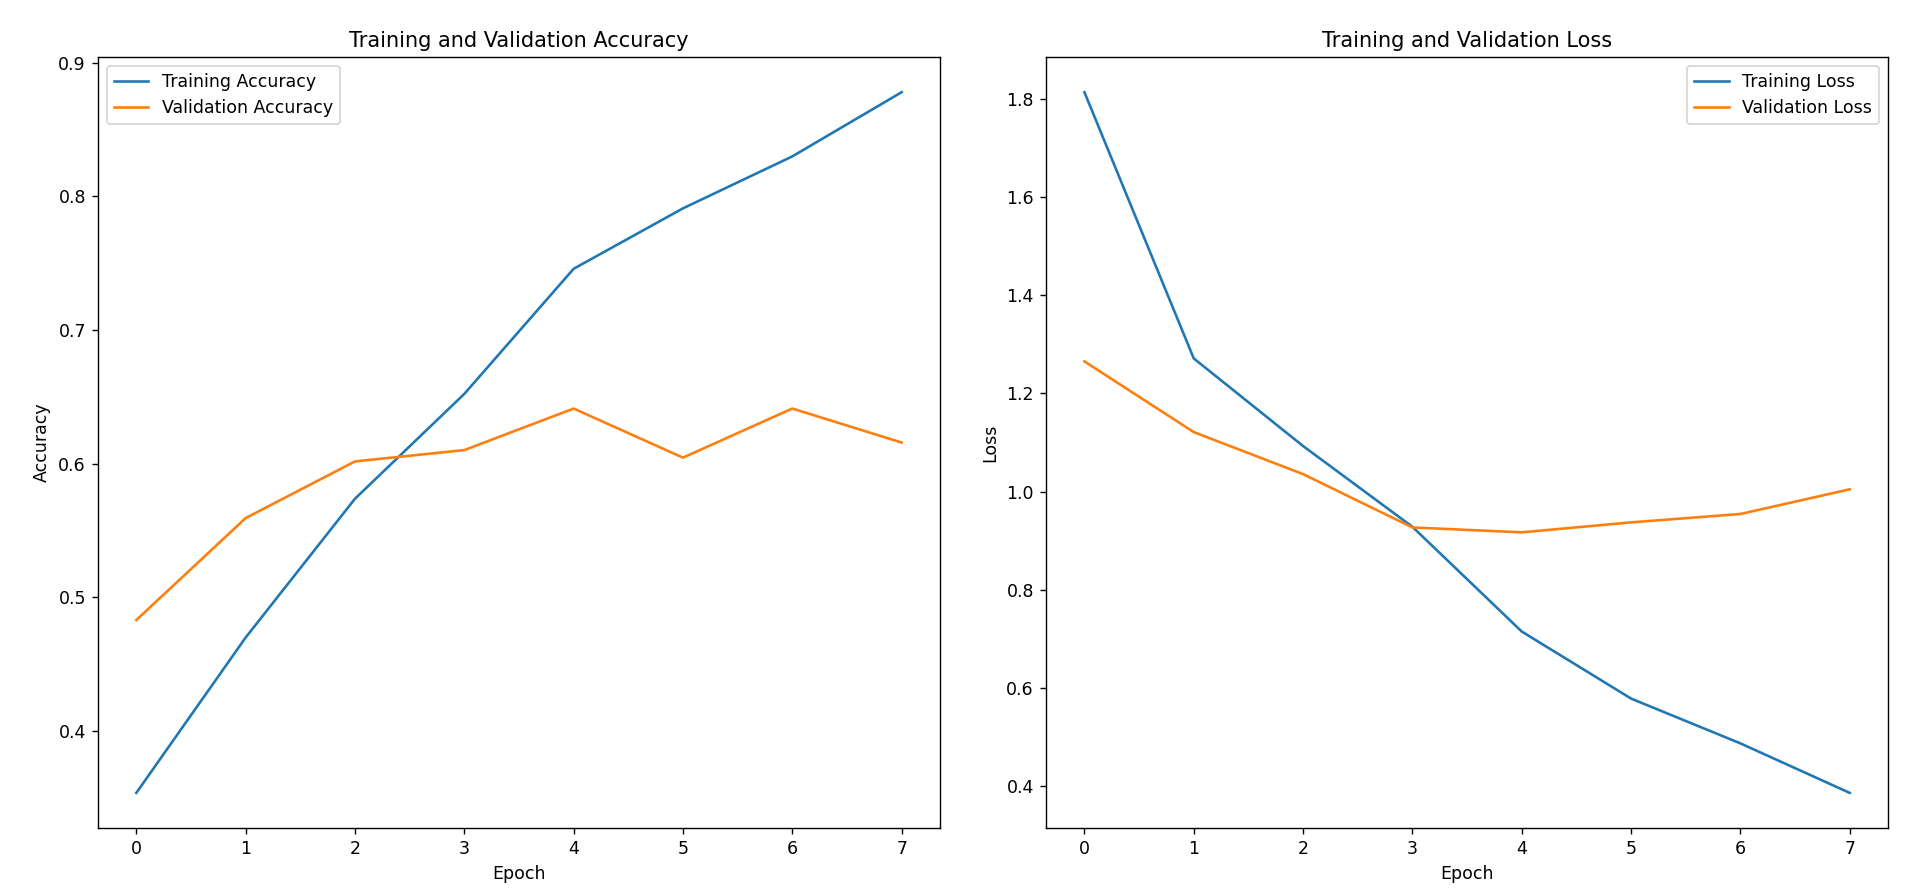
\includegraphics[width=1\textwidth]{results-1.png}
    \caption{Architecture v1 Results}
    \label{fig:results-1}
\end{figure}
In Figure~\ref{fig:results-1} are the results of model architecture v1. The results are slightly better as the validation loss does decrease a little bit (this is likely because of the two extra dropout layers), but still is over-fit.
\begin{figure}[H]
    \centering
    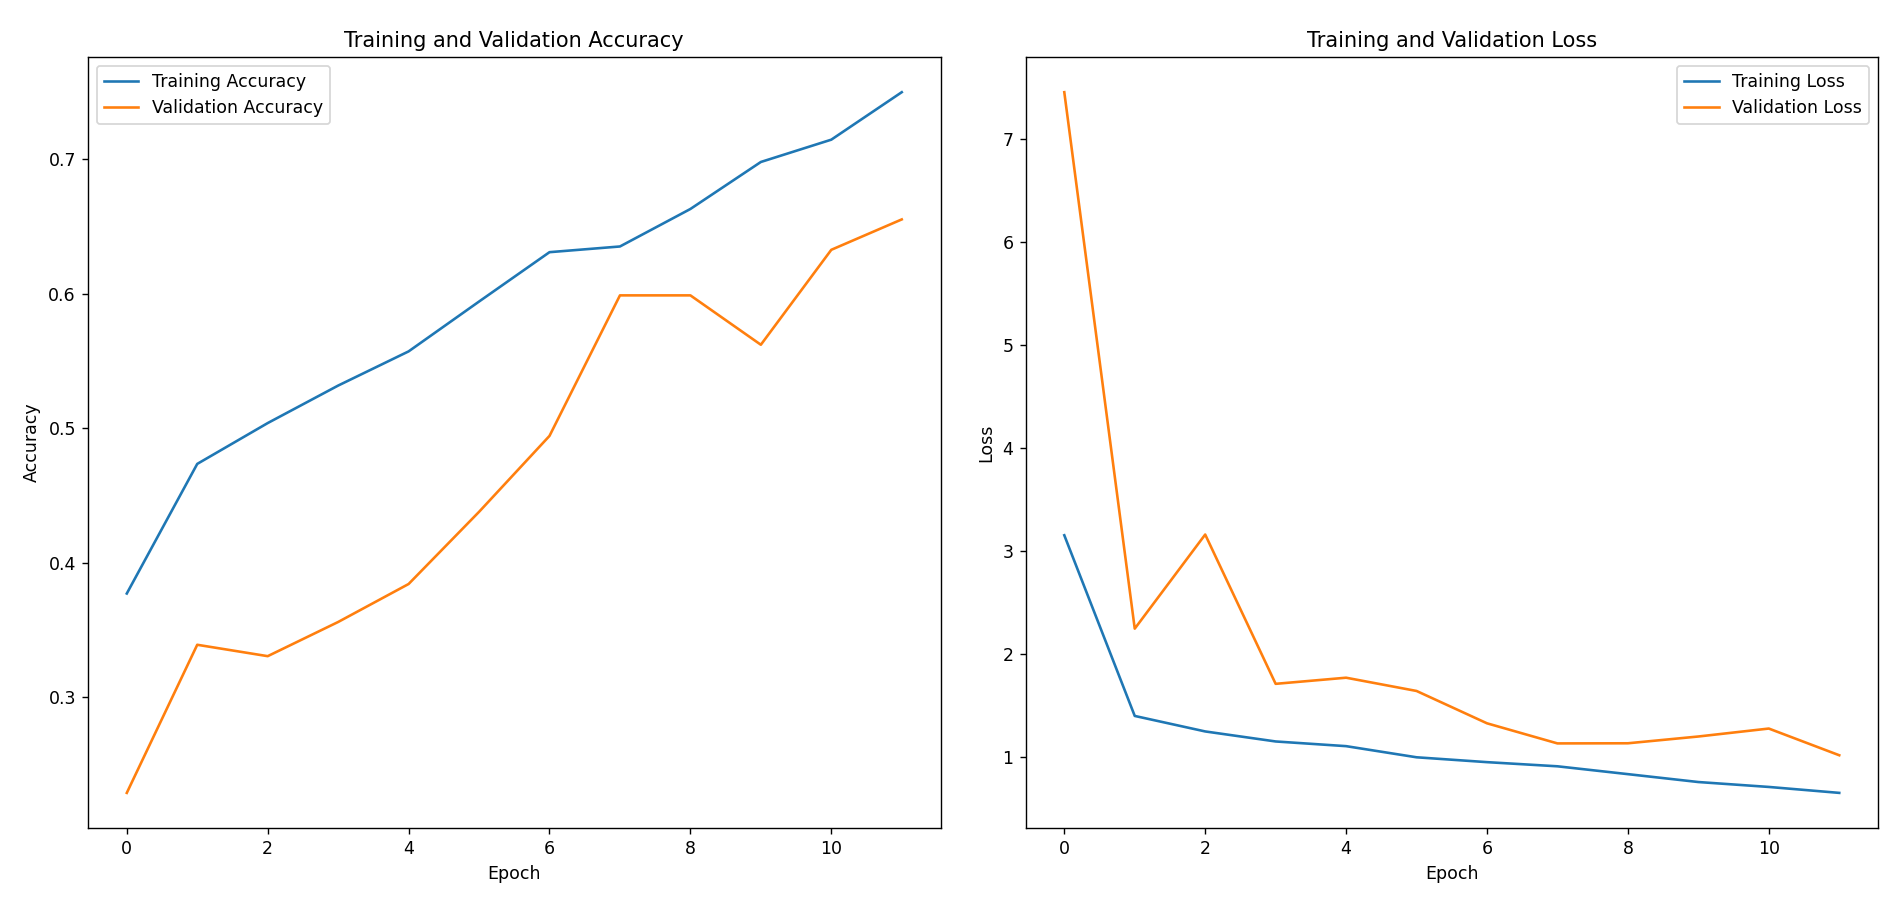
\includegraphics[width=1\textwidth]{results-2.png}
    \caption{Architecture v2 Results}
    \label{fig:results-2}
\end{figure}
In Figure~\ref{fig:results-2} are the results of model architecture v2. This version of the model showed the best results, so I decided to stick with this model for all other testing. The validation loss and accuracy functions closely follow training metrics, which is a sign that the model is not over-fitting.
\begin{figure}[H]
    \centering
    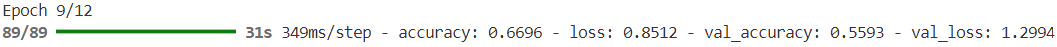
\includegraphics[width=1\textwidth]{gradient-linear.png}
    \caption{Architecture v2 Results With SGD and 'linear'}
    \label{fig:gradient-linear}
\end{figure}
I tried changing the optimization method to gradient descent and activation function to linear and surprisingly the results were really good (Figure~\ref{fig:gradient-linear}).

\section*{Test Set Accuracy and Confusion Matrix}
\begin{figure}[H]
    \centering
    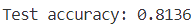
\includegraphics[width=0.5\textwidth]{test-accuracy-2.png}
    \caption{Architecture v2 Test Set Accuracy}
    \label{fig:test-accuracy-2}
\end{figure}
The accuracy (on a test set) of architecture v2 model after 12 epochs of training is 0.8136.
\begin{figure}[H]
    \centering
    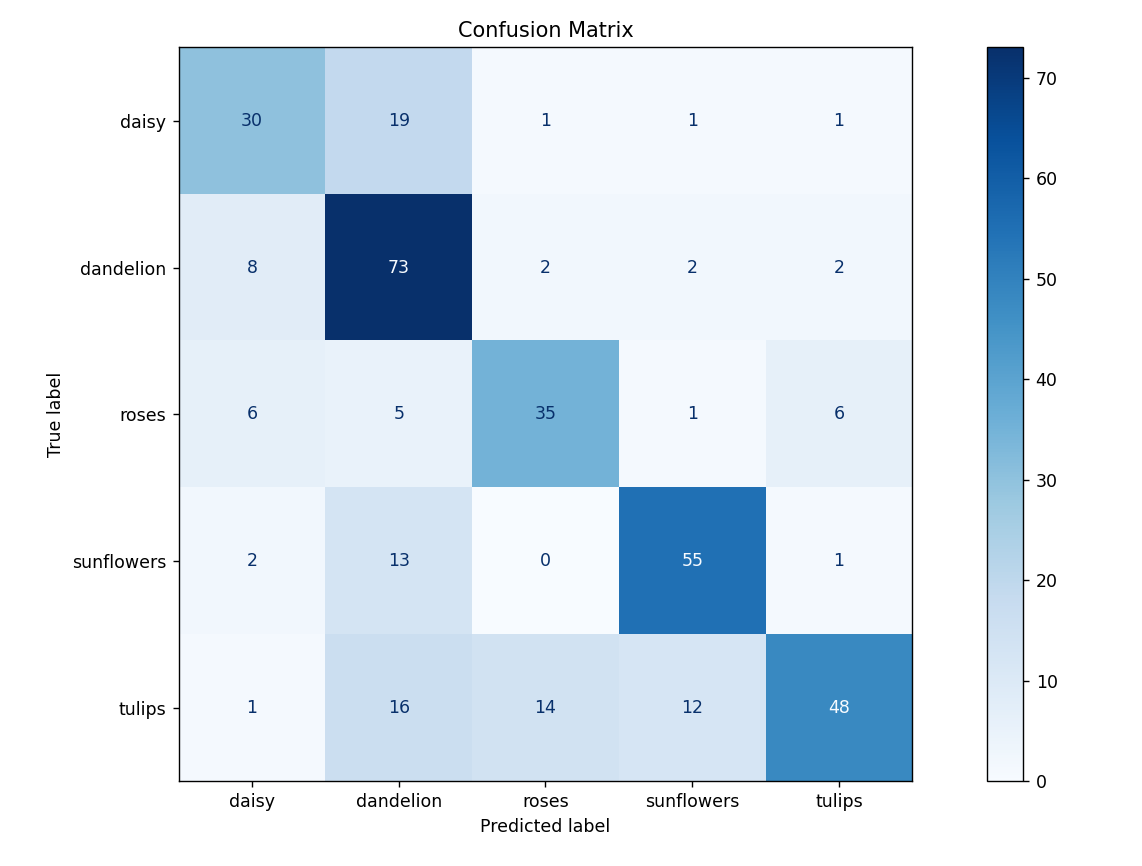
\includegraphics[width=1\textwidth]{confusion-2.png}
    \caption{Architecture v2 Confusion Matrix On Test Set}
    \label{fig:confusion-2}
\end{figure}
Figure~\ref{fig:confusion-2} shows the confusion matrix of test set predictions. The matrix shows good results as most the highest numbers lie on the diagonal. We can also see that the model tends to predict 'dandelion' when the true label is actually 'sunflowers' or 'tulips' or 'daisy'.

\section*{Test Set Predictions}
\begin{table}[H]
    \centering
    \caption{True Labels Compared To Model Predictions}
    \begin{tabular}{|c|c|}
        \hline
        \textbf{True Label} & \textbf{Predicted Label} \\
        \hline
        tulips      & tulips      \\
        daisy       & dandelion   \\
        dandelion   & dandelion   \\
        roses       & tulips      \\
        dandelion   & dandelion   \\
        roses       & roses       \\
        dandelion   & dandelion   \\
        tulips      & tulips      \\
        daisy       & daisy       \\
        daisy       & daisy       \\
        dandelion   & dandelion   \\
        tulips      & tulips      \\
        sunflowers  & sunflowers  \\
        tulips      & roses       \\
        roses       & dandelion   \\
        dandelion   & dandelion   \\
        dandelion   & dandelion   \\
        roses       & roses       \\
        roses       & roses       \\
        dandelion   & dandelion   \\
        roses       & tulips      \\
        dandelion   & dandelion   \\
        daisy       & daisy       \\
        dandelion   & dandelion   \\
        dandelion   & dandelion   \\
        sunflowers  & sunflowers  \\
        dandelion   & dandelion   \\
        sunflowers  & sunflowers  \\
        tulips      & roses       \\
        dandelion   & dandelion   \\
        \hline
    \end{tabular}
    \label{tab:predictions}
\end{table}
Table~\ref{tab:predictions} above compared the true labels of test set to the model predictions.

\section*{Conclusion}
One of the more interesting insights to me was that the model was able to perform with linear activation function after being trained using gradient descent. I always thought that these methods were ineffective for neural networks and that a linear activation function is bad, because it does not introduce non-linearity. Also, using batch normalization and dropout proved to be super effective in combating over-fitting. Another interesting insight is that my computer memory was able to handle the whole dataset of images.

    
\end{document}